\documentclass[a4paper,11pt]{article}
 
\usepackage[english]{babel}
\usepackage[T1]{fontenc}
\usepackage[ansinew]{inputenc}
\usepackage{bbold}
\usepackage{bold-extra}
\usepackage{lmodern}
\usepackage{amsmath}
\usepackage{amsthm}
\usepackage{tkz-berge}
\usepackage{amsfonts}
\usepackage{gensymb}
\usepackage{mathtools}
\usepackage{subfigure}
\usepackage{theorem}
\usepackage{bm}
\usepackage{xcolor}
\usepackage[unicode]{hyperref}
\usepackage{algorithm}
\usepackage{algorithmic}
\usepackage{tikz}
\usepackage{graphicx}
\usepackage{lipsum}
\usetikzlibrary{positioning}
\usepackage{tikz}
\usepackage{empheq}
\usepackage{booktabs}
\usepackage{authblk}
\usetikzlibrary{arrows,shapes}
\usetikzlibrary{arrows}
\usepackage{pdfpages}
\usepackage{wrapfig}



%\usepackage{3dplot} %requires 3dplot.sty to be in same directory, or in your LaTeX installation
%\usepackage{amsmath,amsfonts,amssymb,amsthm,epsfig,epstopdf,titling,url,array}
\usepackage{xstring}

%\theoremstyle{definition}
%\newtheorem{defn}{Definition}[section]
%\newtheorem{conj}{Conjecture}[section]
%\newtheorem{exmp}{Example}[section]
\makeatletter
\newcommand{\change@uppercase@math}{%
  \count@=`\A
  \loop
    \mathcode\count@\count@
    \ifnum\count@<`\Z
    \advance\count@\@ne
  \repeat}

\newcommand{\LSTM}[1]{
  \mathrm{LSTM}(
  %(\begingroup\change@uppercase@math#1\endgroup)
}

\newcommand{\ENC}[1]{
  \mathrm{ENC}(
  %(\begingroup\change@uppercase@math#1\endgroup)
}

\newcommand{\DEC}[1]{
  \mathrm{DEC}(
  %(\begingroup\change@uppercase@math#1\endgroup)
}

\newcommand{\UPDATE}[1]{
  \mathrm{UPDATE}(
  %(\begingroup\change@uppercase@math#1\endgroup)
}

\newcommand{\READ}[1]{
  \mathrm{READ}(
 % (\begingroup\change@uppercase@math#1\endgroup)
}

\newcommand{\CIRC}[1]{
  \mathrm{circ}(
 % (\begingroup\change@uppercase@math#1\endgroup)
}

\newcommand{\RNN}[1]{
  \mathrm{RNN}(
 % (\begingroup\change@uppercase@math#1\endgroup)
}

\newcommand{\ReLU}[1]{
  \mathrm{ReLU}(
 % (\begingroup\change@uppercase@math#1\endgroup)
}


\newcommand{\softmax}[1]{
  \mathrm{softmax}(
 % (\begingroup\change@uppercase@math#1\endgroup)
}


\makeatother

\newcommand*\GetListMember[2]{\StrBetween[#2,\number\numexpr#2+1]{,#1,},,\par}%
\newcommand{\tikzmark}[1]{\tikz[overlay,remember picture] \node (#1) {};}

\def\spvec#1{\left(\vcenter{\halign{\hfil$##$\hfil\cr \spvecA#1;;}}\right)}
\def\spvecA#1;{\if;#1;\else #1\cr \expandafter \spvecA \fi}

\newlength{\MidRadius}
\newcommand*{\CircularSequence}[3]{%
    % #1 = outer circle radius
    % #2 = inner circle radius
    % #3 = seqeunce
    \StrCount{#3}{,}[\NumberOfElements]
    \pgfmathsetmacro{\AngleSep}{360/(\NumberOfElements+1)}
    \pgfmathsetlength{\MidRadius}{(#1+#2)/2}
    \draw [red,  ultra thick] circle (#2);
    \draw [blue, ultra thick] circle (#1);
%    \draw [thick,->] (0, 0) -- (1.0, 0);
%    \draw [thick,->] (0, 0) -- (0.0, 1.0);
    \foreach [count = \Count] \Angle in {0,\AngleSep,..., 360} {%
        \draw [gray, ultra thick] (\Angle:#2) -- (\Angle:#1);
        \pgfmathsetmacro{\MidPoint}{\Angle+\AngleSep/2}
        \node at (\MidPoint:\MidRadius) {\GetListMember{#3}{\Count}};
    }%7
}%


\author{Povilas Daniu\v{s}is, Audrius Indriulionis, Andrius Budrionis}


\title{Computer Vision-based System for Impaired Human Vision Compensation}

\begin{document}
\pgfdeclarelayer{background}
\pgfsetlayers{background,main}


\maketitle


\section{Introduction}
\label{sec:introduction}

More than $250$ million poople worldwide have moderate to severe vision impairment, while ($\approx 36$ million are blind) \cite{Bourne}. During the past decades significant effort was devoted to develop computer vision and other sensor based aids (e.g. \cite{Caraiman}, \cite{Csapo}, \cite{Poggi}, \cite{Zientara}) for helping the blind and visually impaired users to perceive the surrounding world. However, computer vision is rapidly evolving field, and systems based on the aforementioned approaches often lack accuracy and reliability in real-world conditions. In this article we describe a system, which employs modern computer vision techniques for compensation of lost or impaired vision function in humans. Many of the previuosly proposed electronic aids for the blind count on highly specialised hardware, for instance smart glassess \cite{Zientara}, Microsoft Kinnect sensors \cite{Owayjan}, helmet-mounted photosensors and cameras \cite{Larisa}. Such advanced and costly technology brings additional complexity into daily tasks, which visually impaired people currently manage by the help of the white cane. This project puts major emphasis on developing a tool, which seamlesly integrates with the hardware visually impaired person already has on-hand and is used to (smartphone). This paper describes the high level architecture of the proposed technology aid for visually impaired people. 


%The article is organized as follows: in Section~\ref{sec:method} we describe our method, Section~\ref{sec:results} presents the schematic description of human vision compensation system (HVCS). Limitations and further implications of the proposed system are discussed in the Section~\ref{sec:discussion}.


%We assume that mobile device equivalent or very similar to smartphone is used by the visually impaired person to perceive visual information from the environment by inbuilt or auxiliary cameras. Since most of computer vision algorithms require rather intensive computational power exceeding than that of smartphone, we also assume that image processing itself can be conducted in separate machine, connected to the mobile device via Internet, and calculated audio or tactile feedback signal is transmited to the mobile device for presentation to the user. 

%According to \cite{Bourne} more than $250$ million persons have moderate to severe vision impairment ($\approx 36$ million are blind). During past decades significant effort was devoted by various authors to develop computer vision and other sensor based aids (e.g. \cite{Caraiman}, \cite{Csapo}, \cite{Poggi}, \cite{Zientara}) for helping the blind and visually impaired users to perceive the world around. However, computer vision is rapidly evolving field, and systems based on aforementioned approaches often lack accuracy and reliability in real-world conditions. In this article we describe realistic system, which allow to use modern computer vision methods for compensation of lost or impaired vision function in humans. We assume that mobile device equivalent or very similar to smartphone is used to perceive visual information from the environment. Since most of computer vision algorithms require rather intensive computational power exceeding than that of smartphone, we also assume that image processing itself is conducted in separate machine, connected to the mobile device via Internet, and calculated audio or tactile feedback signal is transmited to the mobile device for presentation to the user.

\section{Method}
\label{sec:method}

Following the principles of participatory design \cite{Kensing}, \cite{Carroll} we included the final users into the design process of the system. Two visually impaired persons participated in discussion and focus group meetings together with the project team to identify the key properties of the solution. During the six discussion sessions major attention was paid to:
\begin{enumerate}
\item Functionality and key features of the solution addressing real-life scenarios of visually impaired persons;
\item Technical feasibility, connecting user needs to the latest development in computer vision and assisted technologies;
\item Interface between the visually impaired person and the assisted technology;
\item Appearance, usability and potential costs of the final product. 
\end{enumerate}
Design process involved testing of the existing technological solutions (mobile phone apps) for assisting visually impaired persons {\color{red}(which ones have we tested?)}. Semi-structured tests were performed by the visually impaired participants accompanied by a researcher from a project group. Strengths and weaknesses of the existing solutions are reflected in the design of the proposed system. 


\section{Results}
\label{sec:results}

\begin{wrapfigure}{r}{0.4\textwidth}
  \begin{center}
    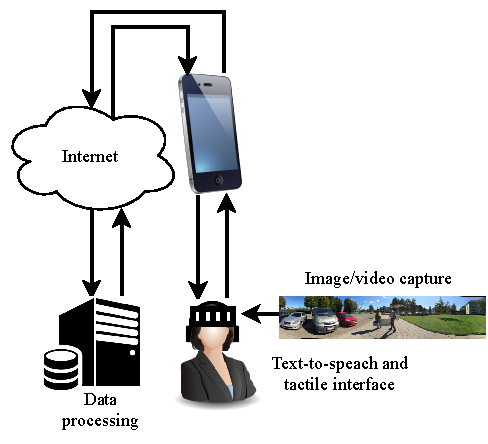
\includegraphics[scale=0.7]{./img/cropped_diagram.pdf}  
  \end{center}
  \caption{Schematics of FRP device.}
  \label{fig:schematics}
\end{wrapfigure}


The key functionality of smart device enables to label the road 'home-office' on the real map that helps  visually impaired community expand the knowledge about the assitive roads for safe navigation. The composed solution of labeled object  location and direction detection assisted by smartphone device enables to trust the new developed technology for visually impaired people.

Technical feasibility
After the survey of visually impaired people needs the authors came to conclusion from 5 to 8 object class should be detected the position and orientation and the key feasibility of device should help to learn the "home-office" road in most efficient way.
The recent developments of computing vision algorithms show the more promising results integrating the smartphone devices for image capturing and preprocessing.  The computational resources are allocated to perform 
%Interface
Light weighted and head mounted tactile device receives the information from server about the object location, including distance and direction to it. The bone headphone device will be used for assistive information provided through internet server...

Following the above methodology we suggest the impaired human vision compensation system (\textbf{HVCS}), consisting of \textbf{Device} and \textbf{Inference} components (see Fig.~\ref{fig:schematics}).

%padalijimas i 2 komponentus man nelabai aiskus. As dalinciau i input (kameros, sensoriai), output (ausines, vibratoriu matricos), processing (local, remote). 
% tai kas dabar yra prie Inference, siulau perprazuot kaip Functionality, ka as minejau Method. Taip pat visa Results skyreli reiktu labiau susiet su Method. Reiktu, kad visi 4 Method pamineti punktai isrysketu ir Results. 
%Results skyrelyje nereiktu taip stipriai fokusuotis i kitu grupiu tyrimus ir juos cituoti. Rezultatai juk musu.
\textbf{Device} subsystem is a computational device the user currently uses for completing other daily tasks. It consists of sensors and actuators, integrated into smartphone-based computation core, which was chosen due its avialability to wide population, and capability to perform the required computations or forward visual information to the external server via Internet connection. Sensors are mounted on forehead belt include: RGB camera, depth camera, IMU. Actuator set consists of bone conductive headphones, and head belt for presenting tactile-feedback to the user. The smartphone device would be integrated with sensors due to capture the street image. The low resources computational device preprocess the image and sends to server to detect the object.  %We suggest to use bone conductive headphones, ... 

\textbf{Inference} subsystem consists of server computer with internet connection and set of computer vision algorithms, selected according to our methodology (see. Sec.~\ref{sec:method}): Faster RCNN object detector \cite{?}, trained to detect important objects (doors, floors, elevators, stairs, corridor junctions, etc.), CNN-RNN-based scene description \cite{Liu},\cite{Ren}, \cite{Dai}, place recognition \cite{Ohn-Bar}, face recognition \cite{Amos}, obstacle detection \cite{Laina}, and possibly other modules. 

HVCS operation cycle is started by \textbf{Device} reading sensor data and transmitting it to the server for an analysis. Server calculates feedback signal and transmits it back to the device for presenting to the user.


\section{Discussion}
\label{sec:discussion}
%Didzioji Discussion teksto dalis man labiau tinka prie Results/Conclusion. Gal galim padiskutioti daugiau apie Limitations, Future Implications, Lessons Learned ar pan... Cia galime savo siuloma sistema lyginti su anksciau publikuotais rezultatais. 

In this article we outlined an idea of computer vision-based sensor, which can help to partially compensate impaired or lost human sight. The developed head-mounted tactile device is developed for head position and orientation tracking and could capture an image in front of visually impaired people. The tactile device with integrated 3D deph camera is integrated with smartphone by bluetooth which could preprocess the labeled image features. The developed high quality self navigation system is based on the computer vision methods especially enhancing the capabilities to detect and classify objects (e.g bus station, street crossings, ) with their surrounding objects. The authors expect to increase the capabilies of potentially blind to secure navigate especially for the planed destination (e.g. "home-office"). 

Work left (outdoor/indoor) etc.


What are main advantages in our proposed solution? What is the reason there is no proposed solution at all?
What exact technical solution should be implemented/developed?
What feasibility and key features are most important for visually impaired people?
\begin{thebibliography}{1}
\bibitem{Amos} Amos, B., Ludwiczuk, B., and Satyanarayanan, M. Openface:
A general-purpose face recognition library with mobile applications. Technical report, CMU-CS-16-118, CMU School of Computer Science, 2016.

\bibitem{Bourne} Bourne RRA, Flaxman SR, Braithwaite T, Cicinelli MV, Das A, Jonas JB, et al.; Vision Loss Expert Group. Magnitude, temporal trends, and projections of the global prevalence of blindness and distance and near vision impairment: a systematic review and meta-analysis. Lancet Glob Health.  2017 Sep;5(9):e888-97.

\bibitem{Caraiman} Caraiman, S., Morar, A., Owczarek, M.,Burlacu, A., Rzeszotarski, D., Botezatu, N., Herghelegiu, P., Moldoveanu, F., Strumillo, P., Moldoveanu, A. Computer Vision for the Visually Impaired: the Sound of Vision System. IEEE International Conference on Computer Vision Workshops, pp. 1480-1489, 2017.
\bibitem{Csapo} Csap\'{o}, A., Wers\'{e}nyi, G., Nagy, H., Stockman, T. A survey of assistive technologies and applications for blind users on mobile platforms: a review and foundation for research. Journal on Multimodal User Interfaces. Vol. 9, issule 4,  pp. 275-286, 2015.
\bibitem{Dai} Dai, J., Li, Y., He, K., Sun J. R-FCN: Object Detection via Region-based Fully Convolutional Networks. In Advances in neural information processing systems, pp. 379-387, 2016.
\bibitem{Poggi} Poggi, M., Mattoccia, S. A wearable mobility aid for the visually impaired based on embedded 3d vision and deep learning. Proceeding of IEEE Symposium on Compututers and Communication, pp. 208-213, 2016.
\bibitem{Zientara} Zientara, P.,A., Lee, S., Smith, G., H., Brenner, R., Itti, L., Rosson M., B., Carroll, J., M., Irick K., M., Narayanan, V. Third Eye: A shopping assistant for the visually impaired. Computer Vol. 50, Issue 2, pp. 16-24, 2017.
\bibitem{Liu} Liu, Ch., Mao, J., Sha, F., Yuille, A. Attention Correctness in Neural Image Captioning. Proceedings of the Thirty-First AAAI Conference on Artificial Intelligence, pp. 4176-4182, 2017.
\bibitem{Laina} Laina, I., Rupprecht, C., Belagiannis, V., Tombari, F., Navab, N. Deeper depth prediction with fully convolutional residual networks. Fourth International Conference on 3D Vision (3DV), pp. 239-248, 2016.
\bibitem{Ohn-Bar}  Ohn-Bar, E., Kitani, K., Asakawa, Ch. Personalized Dynamics Models for Adaptive Assistive Navigation Interfaces. arXiv:1804.04118, [cs.LG], 2018.
\bibitem{Ren} Ren, Sh., He, K., Girshick, R., and Sun, J.  Faster R-CNN: Towards real-time object detection with region proposal networks. In Advances in neural information processing systems, pp. 91-99, 2015.

\bibitem{Kensing} Kensing, F., Simonsen, J., and B\o dker, K. MUST: A Method for Participatory Design. Hum-Comput Interact, vol. 13, no. 2, pp. 167-198, Jun. 1998.

\bibitem{Carroll} Carroll, J. M., Rosson, M. B. Participatory design in community informatics. Des. Stud., vol. 28, no. 3, pp. 243-261, May 2007.

\bibitem{Owayjan} Owayjan, M., Hayek, A., Nassrallah, H., Eldor, M. Smart Assistive Navigation System for Blind and Visually Impaired Individuals. 2015 International Conference on Advances in Biomedical Engineering (ICABME), 2015.

\bibitem{Larisa} Dunai, L. D., Lengua, I. L., Tortajada, I., Brusola Simon, F. Obstacle detectors for visually impaired people. 2014 International Conference on Optimization of Electrical and Electronic Equipment (OPTIM), 2014. 

\end{thebibliography}

\end{document}
